\documentclass[11pt,a4paper]{scrartcl}
%{{{ general stuff
\usepackage[a4paper,bindingoffset=0.2in,%
            left=1in,right=1in,top=1in,bottom=1in,%
            footskip=.25in]{geometry}
\usepackage[english]{babel}
\usepackage[utf8]{inputenc}
\usepackage[T1]{fontenc}
\usepackage{cite}
\usepackage[hidelinks]{hyperref}
\usepackage{float} % use H in figure placement
\pagenumbering{gobble}

%}}}
%{{{ graphics
\usepackage{graphicx} % Bilder
%}}}
%{{{ math
\usepackage{mathrsfs} % mathcal and mathscr
\usepackage{mathtools, amssymb, amsthm}
\usepackage{bm} % cool bold symbols
%}}}
%{{{ a todo command
\newcounter{todocounter}
\newcommand{\todo}[2][noisnotdefined]{
 \marginpar{\fcolorbox{black}{yellow}{\footnotesize\textbf{todo}}
 \ifthenelse{\equal{#1}{noisnotdefined}}{}{\textcolor{black}{\newline\tiny #1}} }
 \textbf{\ifthenelse{\equal{#2}{.}}
   {\fcolorbox{blue}{white}{\textcolor{blue}{$\maltese$} } }{ {\textcolor{blue}{#2} } } }
 \refstepcounter{todocounter} }
%}}}

\date{}
\title{todo: think about good title}
\author{Felix Bartel and D\'avid Kerekes}


\begin{document}

\maketitle

\section{Introduction}

We want to apply a genetic algorithm to a neural network which is known as neuroevolution.
A big advantage of this scheme is that one only needs an indicator how good the neural network performs given a certain task.
This can for instance be given by the outcome of a game.
Our game of choice was Blobby Volley 2 which is a simple two-dimensional volleyball game with open source written in C++ with lua support, see Figure \ref{fig:screenshot}.

\begin{figure}[H]
\center
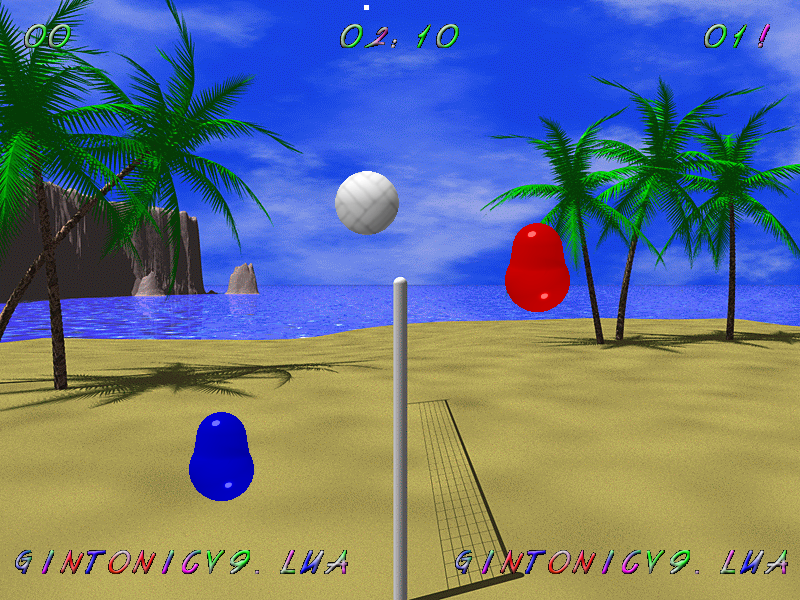
\includegraphics[width=0.4\textwidth]{img/screenshot.png}
\caption{Screenshot of the game.}
\label{fig:screenshot}
\end{figure}

A scene from the game could be described by the $x$- and $y$-coordinates of the players and the ball, their corresponding velocities and the current number of ball contacts.
These arguments or a subset of them could then be used as input for the neural network.
The output would then be the players movement which only consists of going right, left or jumping.
Assuming the layers of the neural network have $n_1,\dots,n_L$ nodes we then have to optimize \[N = \sum_{l=1}^{L-1} (n_l+1) \, n_{l+1}\] number of variables if we fix the size of the network.

The genotype-representation of the network is accomplished through python objects. This will allow a straightforward implementation of a wide variety of genetic operators, while having next to no impact on the speed of training.
As the evaluation of the population is time-consuming, we do this in a thread-parallel fashion, allowing us to exploit multiple high core-count machines at our disposal.


\section{Standard genetic algorithm}

fixed the size of the neural network to $6$ input nodes, one hidden layer with $7$ nodes and $2$ output nodes.


\subsection{Crossover}

As crossover we randomly mixed the nodes with belonging weights and biases of two networks and chose the parents via the fitness proportional roulette wheel selection.


\subsection{Mutation}

Mutation is accomplished by adding Gaussian noise to a subset of all weights and biases.


\subsection{scheme}

Furthermore we implemented elitism.

fitness is the normalized point difference after $21$ serves.

We implemented our own bot to act as an initial trainer \texttt{trainer} for the network.
This trainer is easier to defeat.
We made a copy of each bot where it gives up after a certain amount of touches with the ball, such that normal gameplay will be rewarded.
The simplification gives the evolutionary algorithm the opportunity to start optimizing the neural network in a valid direction, without introducing additional factors to the fitness score.


\subsection{Numerical tests}

\begin{figure}[H]
\center
\begin{tabular}{ccc}
\texttt{reduced} & \texttt{com\_11} & \texttt{gintonicV9} \\
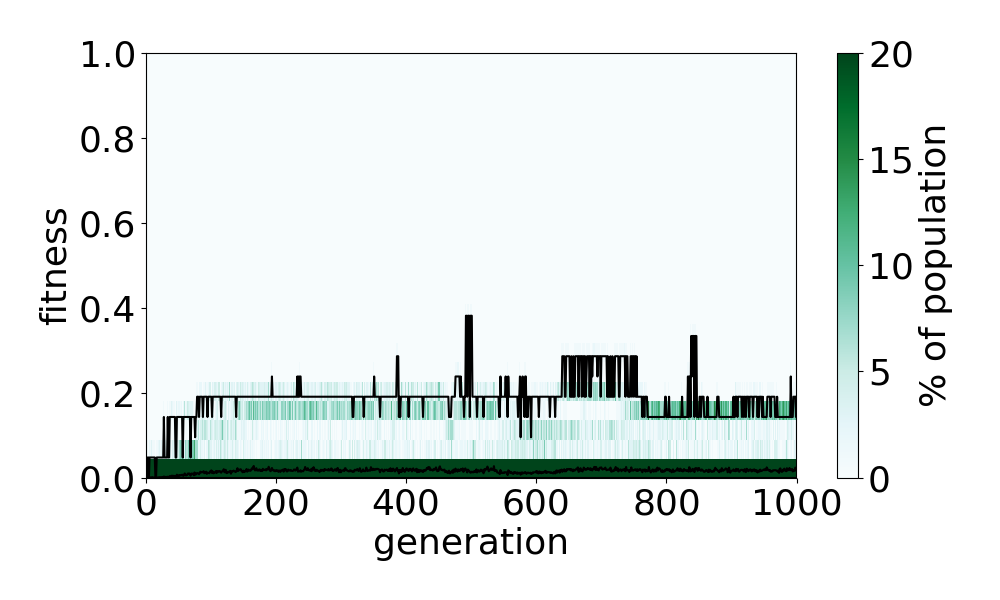
\includegraphics[width=0.3\textwidth]{img/standard_reduced.png} &
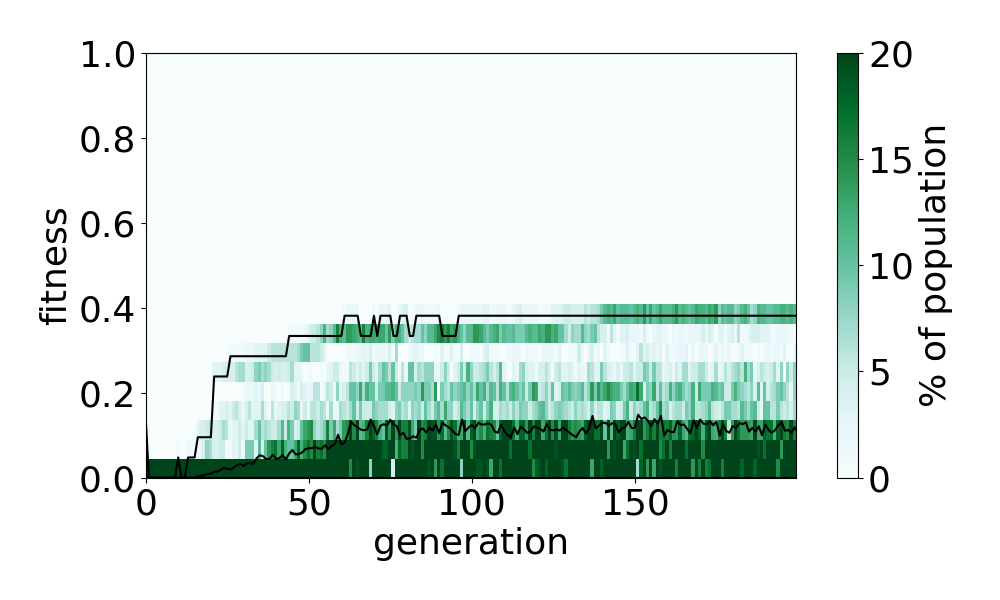
\includegraphics[width=0.3\textwidth]{img/standard_com_11.png} &
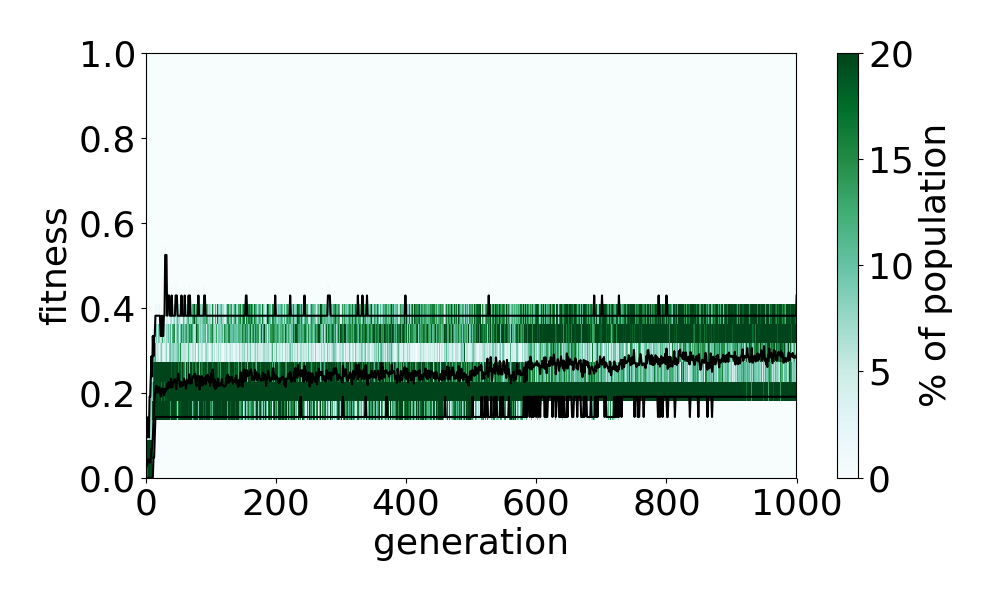
\includegraphics[width=0.3\textwidth]{img/standard_gintonicV9.png} \\
\texttt{hyp014} & \texttt{Union} & \texttt{trainer} \\
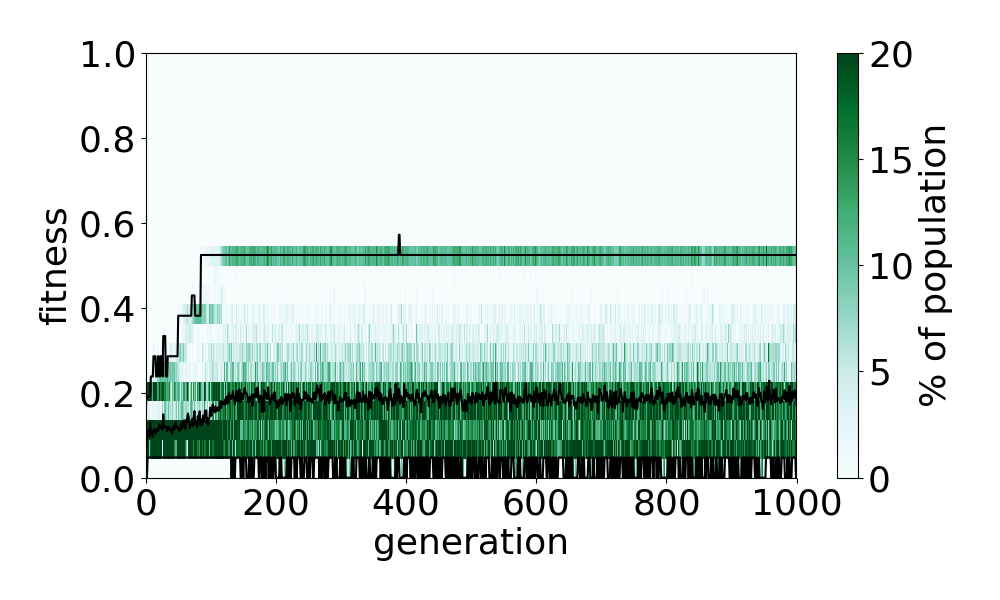
\includegraphics[width=0.3\textwidth]{img/standard_hyp014.png} &
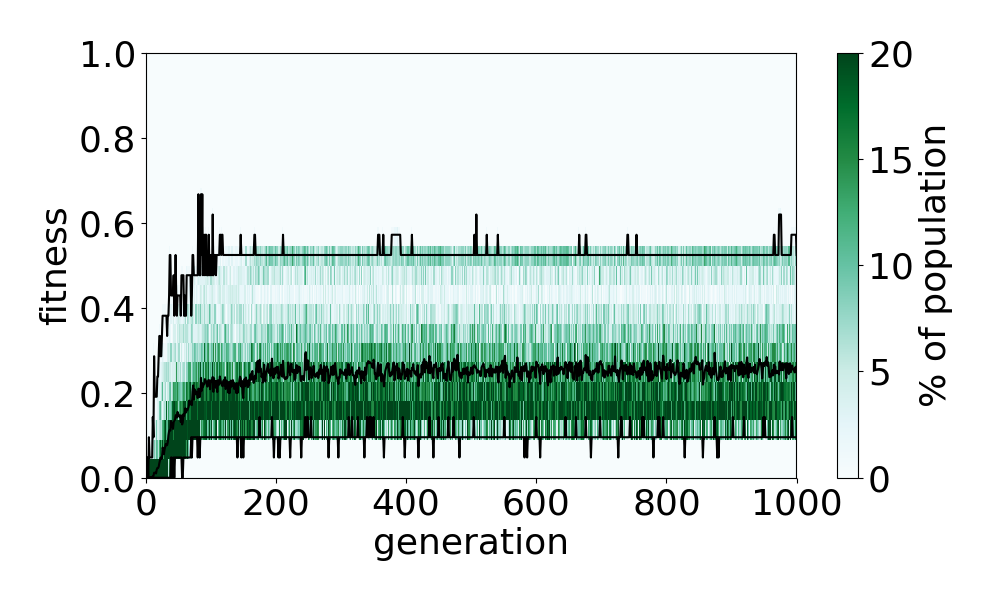
\includegraphics[width=0.3\textwidth]{img/standard_Union.png} &
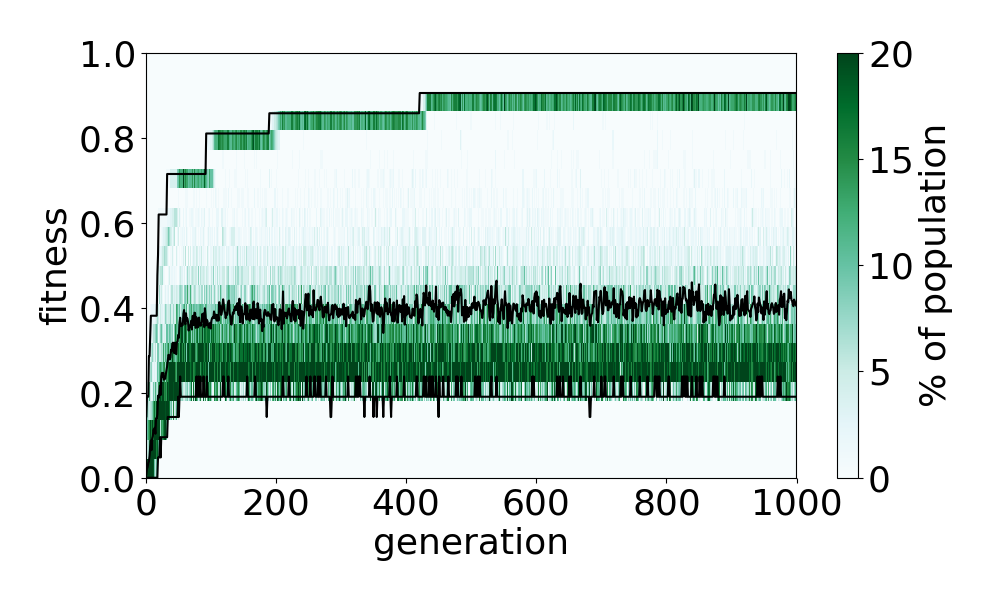
\includegraphics[width=0.3\textwidth]{img/standard_trainer.png}
\end{tabular}
\caption{Fitness density with indicated minimum, average and maximum.}
\label{fig:standard}
\end{figure}


\begin{figure}[H]
\center
\begin{tabular}{ccc}
\texttt{reduced\_5t} & \texttt{com\_11\_5t} & \texttt{gintonicV9\_5t} \\
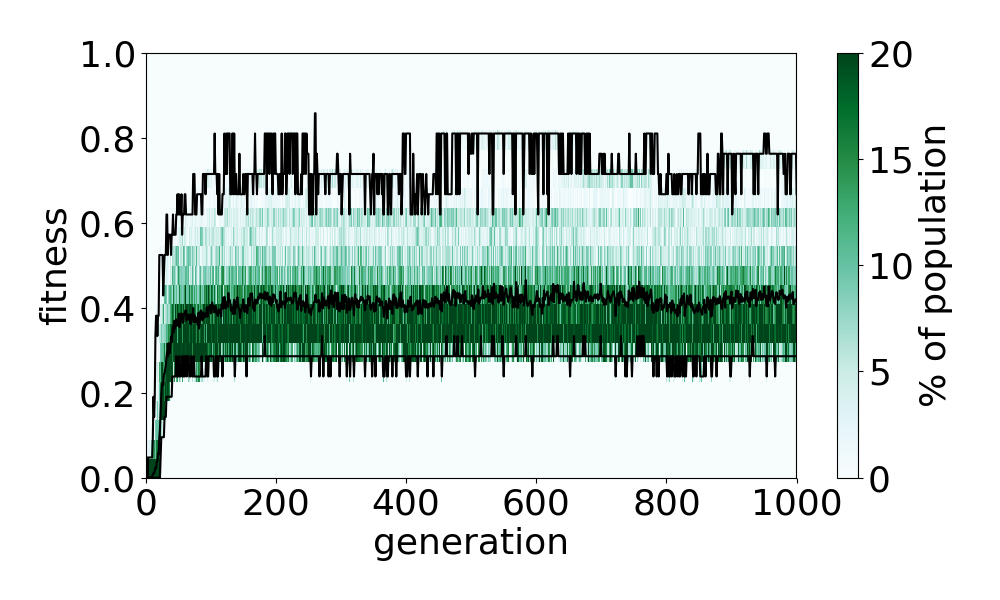
\includegraphics[width=0.3\textwidth]{img/standard_reduced_5t.png} &
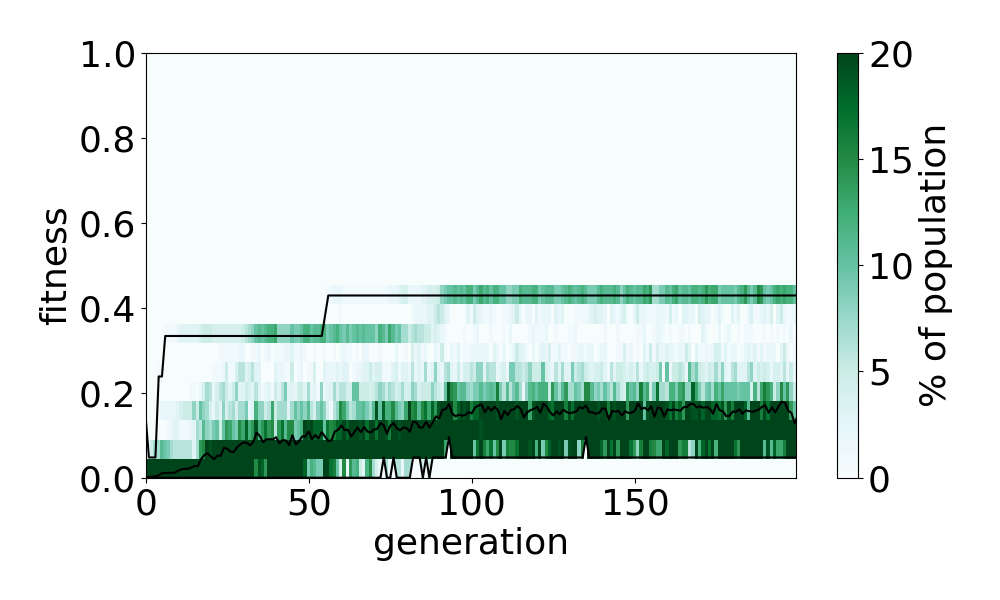
\includegraphics[width=0.3\textwidth]{img/standard_com_11_5t.png} &
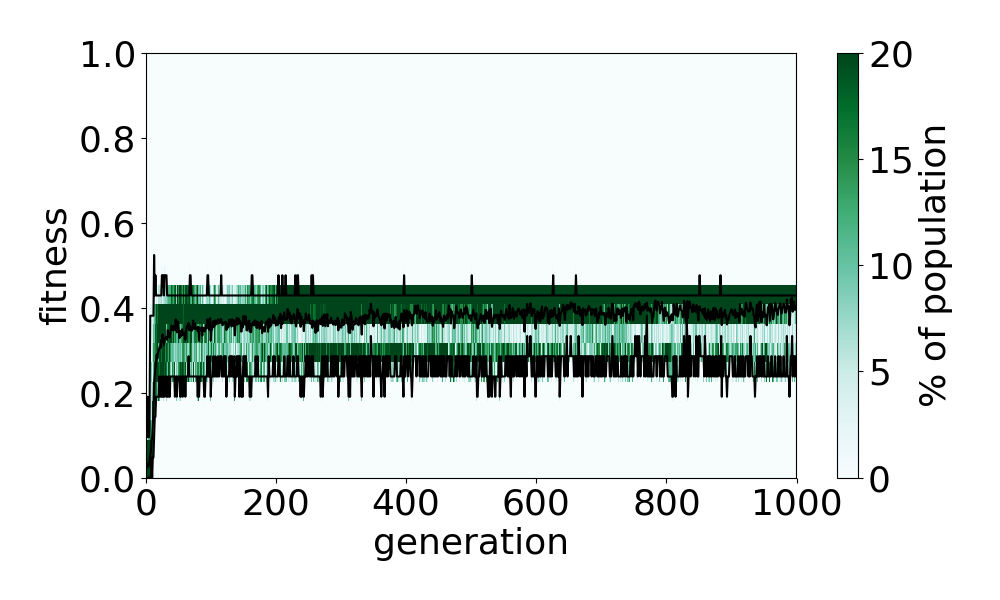
\includegraphics[width=0.3\textwidth]{img/standard_gintonicV9_5t.png} \\
\texttt{hyp014\_5t} & \texttt{Union\_5t} & \texttt{trainer\_5t} \\
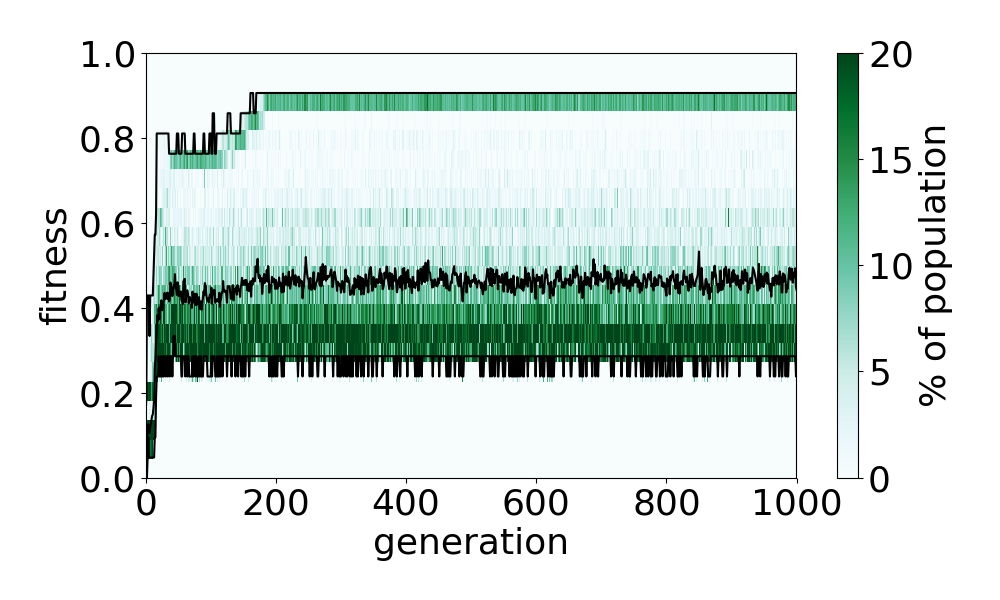
\includegraphics[width=0.3\textwidth]{img/standard_hyp014_5t.png} &
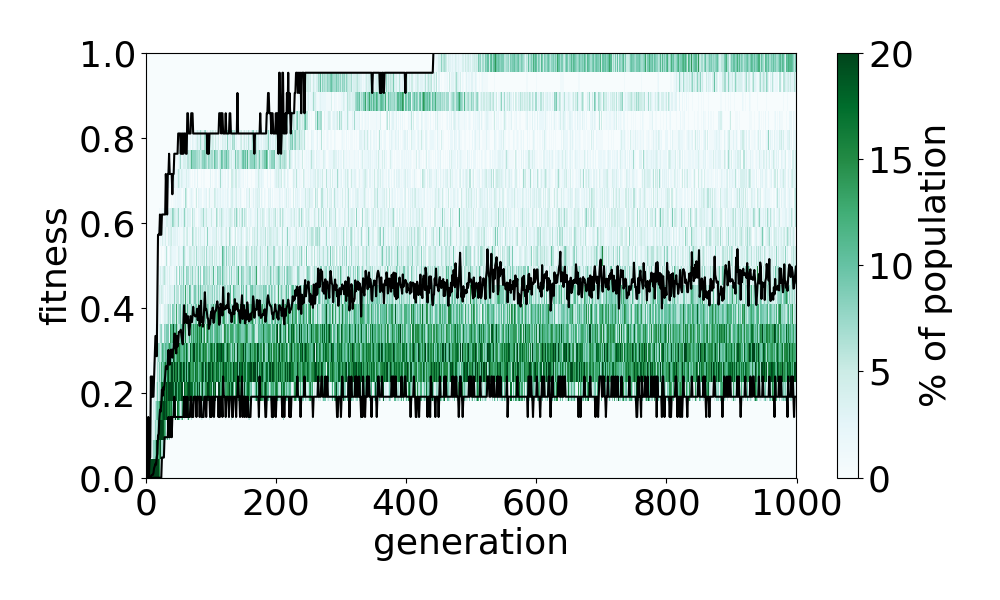
\includegraphics[width=0.3\textwidth]{img/standard_Union_5t.png} &
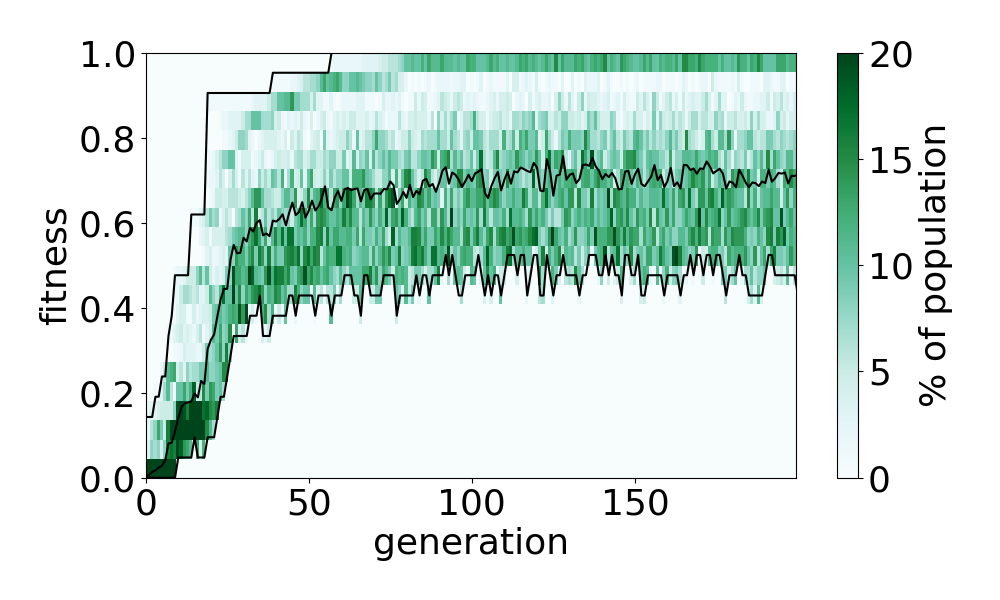
\includegraphics[width=0.3\textwidth]{img/standard_trainer_5t.png}
\end{tabular}
\caption{Fitness density with indicated minimum, average and maximum.}
\label{fig:standard_5t}
\end{figure}


\bibliography{refs}{}
\bibliographystyle{plain}

\end{document}
